\documentclass[ULlof,ULlot]{ULrapport}

% Chargement des packages
\usepackage[utf8]{inputenc}
\usepackage[autolanguage]{numprint}
\usepackage{icomma}
\usepackage{multirow}
\usepackage{tabularx}
\usepackage{pbox}
\usepackage{float}
\usepackage{pifont}

\setcounter{tocdepth}{2}

% Definition d'une commande pour presenter des cellules multilignes dans un tableau
%\newcommand{\cellulemultiligne}[1]{\begin{tabular}{@{}c@{}}#1\end{tabular}}

% Definition de colonnes en mode paragraphe avec alignement ajustable
% Cette definition requiert le chargement du package "array"
%    - alignement horizontal, parametre #1 : - \raggedright (aligne a gauche)
%                                            - \centering (centre)
%                                            - \raggedleft (aligne a droite)
%    - alignement vertical, parametre #2 : - p (aligne en haut)
%                                          - m (centre)
%                                          - b (aligne en bas)
%    - largeur, parametre #3 : longueur
%\newcolumntype{Z}[3]{>{#1\hspace{0pt}\arraybackslash}#2{#3}}

% Page titre
\TitreProjet{Tableau de hockey interactif}
\TitreRapport{Document de conception}
\Destinataire{Martin Savoie}
\NomEquipe{The Javangers}
\TableauMembres{
   111\,127\,868  & Jérémie Bolduc & \\\hline
   111\,126\,228  & Simon-Pierre Deschênes & \\\hline
   111\,121\,082  & Émile Grégoire & \\\hline
   111\,130\,693  & Alexandre McCune & \\\hline
}
\DateRemise{2 octobre 2016}


\HistoriqueVersions{
   0.0 & 19 septembre 2016 & Création du document \\\hline
}

\begin{document}
% Chapitres
\chapter*{Introduction}
\label{s:intro}

Lorem ipsum dolor sit amet, consectetur adipiscing elit. Curabitur odio nisl, feugiat quis quam non, consectetur tempus leo. Etiam nec enim lacus. In porta tempor nisi. Aenean fermentum, sapien at tincidunt pharetra, nibh nunc vehicula urna, sed scelerisque elit risus at ex. Donec egestas, turpis a pellentesque posuere, nibh tellus malesuada elit, sit amet porttitor enim eros a felis. Integer non congue enim. Donec bibendum ex id elementum rutrum. Donec porta nunc et odio gravida, vel vehicula orci aliquet.

Pellentesque gravida fermentum lectus, in laoreet sapien facilisis laoreet. Nunc sit amet leo volutpat, ornare lorem ut, hendrerit ex. Donec lectus augue, interdum in placerat in, dignissim dictum diam. Mauris tincidunt leo nisl, eu convallis odio consectetur id. Vestibulum placerat sem non mattis convallis. Etiam quis lorem imperdiet, gravida felis a, venenatis justo. Praesent eu lorem diam. Phasellus purus mi, tincidunt quis sapien iaculis, eleifend hendrerit est. Sed in justo efficitur, vulputate massa nec, rhoncus tortor. Cras risus nisl, finibus non felis vitae, malesuada sollicitudin ex. Donec finibus sit amet nisi at condimentum. Vivamus vitae libero semper, iaculis orci eget, porttitor sem. Phasellus eget hendrerit mi. Ut feugiat, nulla eu pretium egestas, dui est pretium eros, et tristique ligula magna sed purus
\chapter{Vision}
\label{s:vision}

Lorem ipsum dolor sit amet, consectetur adipiscing elit. Curabitur odio nisl, feugiat quis quam non, consectetur tempus leo. Etiam nec enim lacus. In porta tempor nisi. Aenean fermentum, sapien at tincidunt pharetra, nibh nunc vehicula urna, sed scelerisque elit risus at ex. Donec egestas, turpis a pellentesque posuere, nibh tellus malesuada elit, sit amet porttitor enim eros a felis. Integer non congue enim. Donec bibendum ex id elementum rutrum. Donec porta nunc et odio gravida, vel vehicula orci aliquet.

Pellentesque gravida fermentum lectus, in laoreet sapien facilisis laoreet. Nunc sit amet leo volutpat, ornare lorem ut, hendrerit ex. Donec lectus augue, interdum in placerat in, dignissim dictum diam. Mauris tincidunt leo nisl, eu convallis odio consectetur id. Vestibulum placerat sem non mattis convallis. Etiam quis lorem imperdiet, gravida felis a, venenatis justo. Praesent eu lorem diam. Phasellus purus mi, tincidunt quis sapien iaculis, eleifend hendrerit est. Sed in justo efficitur, vulputate massa nec, rhoncus tortor. Cras risus nisl, finibus non felis vitae, malesuada sollicitudin ex. Donec finibus sit amet nisi at condimentum. Vivamus vitae libero semper, iaculis orci eget, porttitor sem. Phasellus eget hendrerit mi. Ut feugiat, nulla eu pretium egestas, dui est pretium eros, et tristique ligula magna sed purus
\chapter{Modèle des cas d'utilisation}
\label{s:use_cases}
\newpage
\begin{flushleft}
	\textbf{Cas d'utilisation 1 : Créer une stratégie}\\
\end{flushleft}
\begin{tabular}{|p{16cm}|}
	\hline
	\\
	\textbf{Projet :} Visualigue\\
	\\
	\textbf{Niveau :} But d'utilisateur\\
	\\
	\textbf{Acteurs primaires :} Entraineur\\
	\\
	\textbf{Figurants et intérêts :} \\
	- Entraineur: Veut pouvoir créer des fichiers qui contiendront éventuellement des stratégies.\\
	\\
	\textbf{Postconditions :} L'entraineur aura un fichier qui pourra être utilisé pour élaborer une stratégie.\\
	\\
	\textbf{Principal scénario de succès :}\\
	1. Entraineur démarre le processus de création d'une stratégie.\\
	2. Système demande les informations en lien avec la nouvelle stratégie.\\
	3. Entraineur fourni à Système les informations nécessaires.\\
	4. Système demande l'endroit où le fichier devra être enregistré ainsi que le nom de ce dernier.\\
	5. Entraineur choisi l'endroit où le fichier devra être enregistré ainsi que son nom.\\
	6. Système crée le fichier et il est possible de le modifier.\\
	\\
	\textbf{Extensions :}\\
	*a. Entraineur annule le processus de création d'une stratégie.\\
	\hspace{1cm}1. Système demande à Entraineur s'il est certain de vouloir annuler la création d'une stratégie.\\
	\hspace{1cm}2. Entraineur confirme qu'il veut bien annuler la création d'une stratégie.\\
	\hspace{2cm}2a. Entraineur indique qu'il ne veut plus annuler la création d'une stratégie.\\
	\hspace{3cm}1. Système revient où il était dans le processus de création d'une stratégie.\\
	\hspace{1cm}3. Système retourne à la page où il se trouvait avant que le processus de création d'une stratégie ne soit démarré.\\
	1a. Entraineur était au milieu de l'édition d'un fichier.\\
	\hspace{1cm}1. Système demande à Entraineur s'il veut sauvegarder le fichier dont l'édition était en cours.\\
	\hspace{1cm}2. Entraineur choisi s'il veut sauvegarder ou non le fichier dont l'édition était en cours.\\
	5a. Entraineur entre un nom de fichier invalide.\\
	\hspace{1cm}1. Système informe Entraineur que le nom entré est invalide.\\
	\hspace{1cm}2. Entraineur entre un nom valide pour le fichier.\\
	5b. Entraineur choisi un emplacement invalide pour le fichier.\\
	\hspace{1cm}1. Système informe Entraineur que l'emplacement choisi est invalide.\\
	\hspace{1cm}2. Entraineur choisi un emplacement valide pour le fichier.\\
	\\
	\textbf{Fréquence d'occurrence :} Régulièrement\\
	\\
	\textbf{Questions ouvertes :} Quelles seront les informations en lien avec la nouvelle stratégie que l'entraineur devra entrer?\\
	\\
	\hline
\end{tabular}
\newpage
\begin{flushleft}
	\textbf{Cas d'utilisation 2 : Sauvegarder une stratégie}\\
\end{flushleft}
\begin{tabular}{|p{16cm}|}
	\hline
	\\
	\textbf{Projet :} Visualigue\\
	\\
	\textbf{Niveau :} But d'utilisateur\\
	\\
	\textbf{Acteurs primaires :} Entraineur\\
	\\
	\textbf{Figurants et intérêts :} \\
	- Entraineur: Veut pouvoir sauvegarder une stratégie qu'il a élaborée.\\
	\\
	\textbf{Postconditions :} La stratégie est sauvegardée et peut être chargée lors d'une prochaine utilisation du logiciel.\\
	\\
	\textbf{Principal scénario de succès :}\\
	1. Entraineur démarre le processus de sauvegarde de la stratégie.\\
	2. Système sauvegarde la stratégie dans le fichier de stratégie.\\
	\\
	\textbf{Extensions :}\\
	*a. Entraineur annule le processus de sauvegarde d'une stratégie.\\
	\hspace{1cm}1. Système demande à Entraineur s'il est certain de vouloir annuler la sauvegarde d'une stratégie.\\
	\hspace{1cm}2. Entraineur confirme qu'il veut bien annuler la sauvegarde d'une stratégie.\\
	\hspace{2cm}2a. Entraineur indique qu'il ne veut plus annuler la sauvegarde d'une stratégie.\\
	\hspace{3cm}1. Système revient où il était dans le processus de sauvegarde d'une stratégie.\\
	\hspace{1cm}3. Système retourne à la page où il se trouvait avant que le processus de sauvegarde d'une stratégie soit démarré.\\
	\\
	\textbf{Fréquence d'occurrence :} Régulièrement\\
	\\
	\hline
\end{tabular}
\newpage
\begin{flushleft}
	\textbf{Cas d'utilisation 3 : Charger une stratégie}\\
\end{flushleft}
\begin{tabular}{|p{16cm}|}
	\hline
	\\
	\textbf{Projet :} Visualigue\\
	\\
	\textbf{Niveau :} But d'utilisateur\\
	\\
	\textbf{Acteurs primaires :} Entraineur et Joueur\\
	\\
	\textbf{Figurants et intérêts :} \\
	- Entraineur: Veut pouvoir charger une stratégie qu'il a élaborée.\\
	- Joueur: Veut pouvoir charger une stratégie élaborée par l'entraineur.\\
	\\
	\textbf{Postconditions :} La stratégie est chargée et elle peut être modifiée ou visualisée.\\
	\\
	\textbf{Principal scénario de succès :}\\
	1. Entraineur ou Joueur démarre le processus de chargement de la stratégie.\\
	2. Système demande lequel des fichiers de stratégie charger.\\
	3. Entraineur ou Joueur choisi lequel des fichiers de stratégie charger.\\
	4. Système charge le fichier.\\
	\\
	\textbf{Extensions :}\\
	*a. Entraineur ou Joueur annule le processus de chargement d'une stratégie.\\
	\hspace{1cm}1. Système demande à Entraineur ou Joueur s'il est certain de vouloir annuler le chargement d'une stratégie.\\
	\hspace{1cm}2. Entraineur ou Joueur confirme qu'il veut bien annuler le chargement d'une stratégie.\\
	\hspace{2cm}2a. Entraineur ou Joueur indique qu'il ne veut plus annuler le chargement d'une stratégie.\\
	\hspace{3cm}1. Système revient où il était dans le processus de chargement d'une stratégie.\\
	\hspace{1cm}3. Système retourne à la page où il se trouvait avant que le processus de chargement d'une stratégie ne soit démarré.\\
	1a. Entraineur était au milieu de l'édition d'un fichier.\\
	\hspace{1cm}1. Système demande à Entraineur s'il veut sauvegarder le fichier dont l'édition était en cours.\\
	\hspace{1cm}2. Entraineur choisi s'il veut sauvegarder ou non le fichier dont l'édition était en cours.\\
	3a. Entraineur ou Joueur choisi un fichier invalide.\\
	\hspace{1cm}1. Système informe Entraineur ou Joueur que le fichier choisi est invalide.\\
	\hspace{1cm}2. Entraineur ou Joueur choisi un fichier valide.\\
	\\
	\textbf{Fréquence d'occurrence :} Régulièrement\\
	\\
	\hline
\end{tabular}

\newpage
\begin{flushleft}
	\textbf{Cas d'utilisation 4 : Visualiser une stratégie}\\
\end{flushleft}
\begin{tabular}{|p{16cm}|}
	\hline
	\\
	\textbf{Projet :} Visualigue\\
	\\
	\textbf{Niveau :} But d'utilisateur\\
	\\
	\textbf{Acteurs primaires :} Entraineur et Joueur\\
	\\
	\textbf{Figurants et intérêts :} \\
	- Entraineur: Veut pouvoir visualiser une stratégie qu'il a créer.\\
	- Joueur: Veut pouvoir visualiser une stratégie à apprendre.\\
	\\
	\textbf{Principal scénario de succès :}\\
	1. Entraineur ou Joueur démarre le processus de visualisation de la stratégie.\\
	2. Système calcul la position des éléments et les affiches.\\
	\hspace{1cm} \em Système répète l'action 2 jusqu'à la fin de la stratégie.
	\\
	\textbf{Extensions :}\\
	\\
	\textbf{Fréquence d'occurrence :} Régulièrement\\
	\\
	\hline
\end{tabular}

\newpage
\begin{flushleft}
	\textbf{Cas d'utilisation 6 : Placer les éléments}\\
\end{flushleft}
\begin{tabular}{|p{16cm}|}
	\hline
	\\
	\textbf{Projet :} Visualigue\\
	\\
	\textbf{Niveau :} But d'utilisateur\\
	\\
	\textbf{Acteurs primaires :} Entraineur\\
	\\
	\textbf{Figurants et intérêts :} \\
	- Entraineur: Veut pouvoir placer les éléments sur la stratégie et les modifier à sa guise.\\
	\\
	\textbf{Postconditions :} Les éléments sont placés selon ce que l'entraineur souhaite.\\
	\\
	\textbf{Principal scénario de succès :}\\
	1. Entraineur sélectionne un élément de la liste d'éléments disponibles.\\
	2. Système crée un élément selon les spécifications définies dans le sport.\\
	3. Entraineur clique dans l'aire de jeu à l'endroit où l'élément doit être placé.\\
	4. Système place l'élément sur l'aire de jeu et affiche l'élément.\\
	5. Système met à jour la disponibilité de l'élément dans la liste d'éléments disponibles (si nécessaire)\\
	\\
	\textbf{Extensions :}\\
	*a. Entraineur annule le placement de l'élément.\\
	\hspace{0.5cm}1. Système demande à Entraineur s'il est certain de vouloir annuler le placement de l'élément.\\
	\hspace{0.5cm}2. Entraineur confirme qu'il veut bien annuler le placement de l'élément.\\
	\hspace{1cm}2a. Entraineur indique qu'il ne veut plus annuler le placement de l'élément.\\
	\hspace{1.5cm}1. Système revient où il était dans le processus de placement d'un élément.\\
	\hspace{0.5cm}3. Système supprime l'élément créé et réinitialise sa disponibilité (si nécessaire) dans la liste des éléments.\\
	5a. Entraineur souhaite modifier la position de l'élément après l'avoir placé.\\
	\hspace{0.5cm}1. Entraineur clique sur l'élément à modifier.\\
	\hspace{0.5cm}2. Système indique visuellement que l'élément est sélectionné et charge la fenêtre Propriétés avec les paramètres associés.\\
	\hspace{0.5cm}3. Entraineur déplace avec la souris l'élément en question ou modifie la propriété "Position" des paramètres.\\
	\hspace{0.5cm}4. Système déplace l'élément selon les spécifications de l'Entraineur.\\
	5b. Entraineur souhaite modifier la rotation de l'élément.\\
	\hspace{0.5cm}1. Entraineur clique sur l'élément à modifier.\\
	\hspace{0.5cm}2. Système indique visuellement que l'élément est sélectionné et charge la fenêtre Propriétés avec les paramètres associés.\\
	\hspace{0.5cm}3. Système affiche une flèche de rotation près de l'élément sélectionné.\\
	\hspace{0.5cm}4. Entraineur déplace la flèche de rotation jusqu'à l'angle souhaité ou modifie la propriété "Rotation" des paramètres.\\
	\hspace{0.5cm}5. Système oriente l'élément selon les spécifications de l'Entraineur.\\
	5c. Entraineur souhaite modifier le rôle d'un l'élément de type "Joueur".\\
	\hspace{0.5cm}1. Entraineur clique sur l'élément à modifier.\\
	\hspace{0.5cm}2. Système indique visuellement que l'élément est sélectionné et charge la fenêtre Propriétés avec les paramètres associés.\\
	\hspace{0.5cm}3. Entraineur sélectionne le rôle du joueur à partir d'une liste déroulante dans la fenêtre Propriétés.\\
	\hspace{0.5cm}4. Système modifie l'élément pour correspondre aux spécifications du rôle du joueur.\\
	\\
	\textbf{Fréquence d'occurrence :} Régulièrement\\
	\\
	\hline
\end{tabular}

\newpage
\begin{flushleft}
	\textbf{Cas d'utilisation 9 : Exporter une stratégie en format image}\\
\end{flushleft}
\begin{tabular}{|p{16cm}|}
	\hline
	\\
	\textbf{Projet :} Visualigue\\
	\\
	\textbf{Niveau :} But d'utilisateur\\
	\\
	\textbf{Acteurs primaires :} Entraineur\\
	\\
	\textbf{Figurants et intérêts :} \\
	- Entraineur: Veut pouvoir exporter les fichiers de l'applications en image.\\
	\\
	\textbf{Principal scénario de succès :}\\
	1. Entraineur démarre le processus d'exportation.\\
	2. Système demande en quel format les fichiers doivent être exporter.\\
	3. Entraineur sélectionne un format d'image.\\
	4. Système enregistre la stratégie sous forme d'image.\\
	\\
	\textbf{Extensions :}\\
	\\
	\textbf{Fréquence d'occurrence :} Parfois\\
	\\
	\hline
\end{tabular}

\newpage
\begin{flushleft}
	\textbf{Cas d'utilisation 2 : Sauvegarder une stratégie}\\
\end{flushleft}
\begin{tabular}{|p{16cm}|}
	\hline
	\\
	\textbf{Projet :} Visualigue\\
	\\
	\textbf{Niveau :} But d'utilisateur\\
	\\
	\textbf{Acteurs primaires :} Entraineur\\
	\\
	\textbf{Figurants et intérêts :} \\
	- Entraineur: Veut pouvoir sauvegarder une stratégie qu'il a élaborée.\\
	\\
	\textbf{Postconditions :} La stratégie est sauvegardée et peut être chargée lors d'une prochaine utilisation du logiciel.\\
	\\
	\textbf{Principal scénario de succès :}\\
	1. Entraineur démarre le processus de sauvegarde de la stratégie.\\
	2. Système sauvegarde la stratégie dans le fichier de stratégie.\\
	\\
	\textbf{Extensions :}\\
	*a. Entraineur annule le processus de sauvegarde d'une stratégie.\\
	\hspace{1cm}1. Système demande à Entraineur s'il est certain de vouloir annuler la sauvegarde d'une stratégie.\\
	\hspace{1cm}2. Entraineur confirme qu'il veut bien annuler la sauvegarde d'une stratégie.\\
	\hspace{2cm}2a. Entraineur indique qu'il ne veut plus annuler la sauvegarde d'une stratégie.\\
	\hspace{3cm}1. Système revient où il était dans le processus de sauvegarde d'une stratégie.\\
	\hspace{1cm}3. Système retourne à la page où il se trouvait avant que le processus de sauvegarde d'une stratégie soit démarré.\\
	\\
	\textbf{Fréquence d'occurrence :} Régulièrement\\
	\\
	\hline
\end{tabular}


\newpage
\begin{flushleft}
	\textbf{Cas d'utilisation 7 : Configurer les types de sports}\\
\end{flushleft}
\begin{tabular}{|p{16cm}|}
	\hline
	\\
	\textbf{Projet :} Visualigue\\
	\\
	\textbf{Niveau :} But d'utilisateur\\
	\\
	\textbf{Acteurs primaires :} Entraineur\\
	\\
	\textbf{Figurants et intérêts :} \\
	- Entraineur: Veut pouvoir créer et modifier les types de sports supporter par le logiciel.\\
	\\
	\textbf{Postconditions :} Une fois qu'un type de sport est créé, il est possible de créer une stratégie pour ce type de sport et de configurer les obstacles associés à ce type de sport.\\
	\\
	\textbf{Garanties en cas de succès :} Le type de sport a été enregistré.\\
	\\
	\textbf{Principal scénario de succès :}\\
	1. Entraineur démarre le processus de configuration d'un  type de sport.\\
	2. Système demande lequel des types de sport l'utilisateur veut configurer ou s'il veut en créer un nouveau type de sport.\\
	3. Entraineur indique le type à configurer.\\
	4. Système offre de modifier les spécifications du type de sport, telle que le nom du sport, l'imgae pour représenter le terrain, les dimensions réelles du terrain, le nombre de joueurs et les catégories de joueurs associées au sport.\\
	5. Entraineur modifie des spécifications du type de sport.\\
	6. Entraineur démarre le processus d'enregistrement.\\
	7. Système valide et enregistre les modifications du type de sport.\\
	\\
	\textbf{Extensions :}\\
	*a. Entraineur annule le processus de configuration du type de sport.\\
	\hspace{1cm}1. Système demande à Entraineur s'il est certain de vouloir annuler la configuration du type de sport.\\
	\hspace{1cm}2. Entraineur confirme qu'il veut bien annuler la configuration du type de sport.\\
	\hspace{2cm}2a. Entraineur indique qu'il ne veut plus annuler la configuration du type de sport.\\
	\hspace{3cm}1. Système revient où il était dans le processus de configuration.\\
	\hspace{1cm}3. Système retourne à la page où il se trouvait avant que le processus de configuration ne soit démarré.\\
	3a. Entraineur indique qu'il veut créer un nouveau type de sport.\\
	\hspace{1cm}1. Système demande à Entraineur de remplir tout les champs de spécification du type de sport.\\
	\hspace{1cm}2. Entraineur entre toutes les spécifications du type de sport.\\
	\hspace{1cm}3. Entraineur démarre le processus d'enregistrement.\\
	\hspace{1cm}4. Système valide et enregistre la création du type de sport.\\
	7a. Système valide les modifications et constate des données invalides.\\
	\hspace{1cm}1. Système affichae un message d'erreur à l'utlisateur et demande de corriger les données invalides.\\
	\hspace{1cm}2. Entraineur corrige les données.\\
	\\
	\textbf{Fréquence d'occurrence :} Parfois\\
	\\
	\hline
\end{tabular}

\newpage
\begin{flushleft}
	\textbf{Cas d'utilisation 8 : Configurer les obstacles}\\
\end{flushleft}
\begin{tabular}{|p{16cm}|}
	\hline
	\\
	\textbf{Projet :} Visualigue\\
	\\
	\textbf{Niveau :} But d'utilisateur\\
	\\
	\textbf{Acteurs primaires :} Entraineur\\
	\\
	\textbf{Figurants et intérêts :} \\
	- Entraineur: Veut pouvoir créer et modifier les types de sports supporter par le logiciel.\\
	\\
	\textbf{Préconditions :} Un type de sport a été créé.\\
	\\
	\textbf{Garanties en cas de succès :} Les obstacles ont été enregistré.\\
	\\
	\textbf{Principal scénario de succès :}\\
	1. Entraineur démarre le processus de configuration des obstacles.\\
	2. Système demande pour lequel des types de sport l'utilisateur veut configurer les obstacles.\\
	3. Entraineur indique le type désiré.\\
	4. Système offre d'ajouter, de modifier ou de supprimer un obsatce.\\
	5. Entraineur choisi de modifier les spécifications d'un obstacle.\\
	6. Système offre de modifier les spécifications de l'obstacle, telle que le nom de l'obstacle, l'imgae pour représenter l'obstacle et les dimensions réelles de l'obstacle.\\
	7. Entraineur modifie des spécifications de l'obstacle.\\
	8. Entraineur démarre le processus d'enregistrement.\\
	9. Système valide et enregistre les modifications de l'obstacle.\\
	\\
	\textbf{Extensions :}\\
	*a. Entraineur annule le processus de configuration de l'obstacle.\\
	\hspace{1cm}1. Système demande à Entraineur s'il est certain de vouloir annuler la configuration de l'obstacle.\\
	\hspace{1cm}2. Entraineur confirme qu'il veut bien annuler la configuration de l'obstacle.\\
	\hspace{2cm}2a. Entraineur indique qu'il ne veut plus annuler la configuration de l'obstacle.\\
	\hspace{3cm}1. Système revient où il était dans le processus de configuration.\\
	\hspace{1cm}3. Système retourne à la page où il se trouvait avant que le processus de configuration ne soit démarré.\\
	5a. Entraineur indique qu'il veut créer un nouvelle obstacle.\\
	\hspace{1cm}1. Système demande à Entraineur de remplir tout les champs de spécification de l'obstacle.\\
	\hspace{1cm}2. Entraineur entre toutes les spécifications de l'obstacle.\\
	\hspace{1cm}3. Entraineur démarre le processus d'enregistrement.\\
	\hspace{1cm}4. Système valide et enregistre la création du type de sport.\\
	5b. Entraineur indique qu'il veut supprimer un obstacle.\\
	\hspace{1cm}1. Système demande à Entraineur de confimer son choix.\\
	\hspace{1cm}2. Entraineur confirme qu'il veut bien supprimer l'obstacle.\\
	\hspace{2cm}2a. Entraineur indique qu'il ne veut plus supprimer l'obstacle.\\
	\hspace{3cm}1. Système revient à l'interface d'ajout/modification/suppression.\\
	\hspace{1cm}3. Système supprime l'obstacle et revient à l'interface d'ajout/modification/suppression.\\
	9a. Système valide les modifications et constate des données invalides.\\
	\hspace{1cm}1. Système affichae un message d'erreur à l'utlisateur et demande de corriger les données invalides.\\
	\hspace{1cm}2. Entraineur corrige les données.\\
	\\
	\textbf{Fréquence d'occurrence :} Parfois\\
	\\
	\hline
\end{tabular}
\chapter{Spécifications supplémentaires}
\label{s:supplementary_specification}
\section{Fonctionnalité}

\subsection{Annuler/Rétablir}
Permet à l'utilisateur d'annuler les dernières actions effectuées durant les modifications apportées à une stratégie. Permet aussi de rétablir les dernières actions qui ont été annulées.

\subsection{Afficher les coordonnées de la sourie}
En tout temps durant la modification d'une stratégie, affiche la position de la souris en unité réelles.

\subsection{Gestion des erreurs}
À tout moment, indique à l'utilisateur la cause des erreurs et la marche a suivre (lorsque nécessaire).



\section{Convivialité}

\subsection{Facteur humain}
Une partie des utilisateurs seront de jeunes enfants avec peu d'expérience avec ce genre de système. Ainsi, l'interface de visualisation de stratégie sera conçu pour être intutive afin de facilité l'utilisation de l'application pour les jeunes joueurs. Pour se faire, les fonctionnalités seront clairement affichées et expliquées au besoin.



\section{Supportabilité}

\subsection{Adaptabilité}
Une telle application peut s'avéré utile pour plus de sport que seulement le hockey. Ainsi, il est possible de confirgurer les types de sport et les obstacles supporter par l'application afin de s'adapté à tout les sports et à tout les types d'entrainnements.









\chapter{Modèle du domaine}
\label{s:domain_model}

Cette section présente le modèle du domaine de VisuaLigue. La figure \ref{fig:domain_model} présente une vue globale de l'application.

\begin{figure}[H]
	\centering
	\includegraphics[width=\textwidth]{{"fig/diagrams/Modele du domaine"}.png}
	\caption{Diagramme du modèle du domaine}
	\label{fig:domain_model}
\end{figure}

Le point d'entrée est l'utilisateur. Celui-ci peut être un Entraineur, un Joueur ou un Parent. Dans ce diagramme, on prend en considération que l'utilisateur est un Entraineur, car il peut exécuter toutes les actions.

L'utilisateur peut configurer des sports. Un sport est constitué d'un terrain, de plusieurs descriptions de joueurs, de balles et d'obstacles. Le terrain contient l'image, la taille et les dimensions. Il ne peut y avoir qu'un seul terrain par sport. Les descriptions des joueurs, des balles et des obstacles contiennent les propriétés qui seront utilisées lors de l'ajout de ceux-ci dans une stratégie. Par exemple, c'est ici que l'on définit le rôle des joueurs. Puisque plusieurs propriétés sont partagées entre ces classes, une généralisation appelée \textit{DescriptionÉlément} a été créée. Afin d'alléger le diagramme, la classe utilisateur n'a pas été reliée aux descriptions ni au terrain. Toutefois, on comprendra que lorsque l'utilisateur configure un sport, il modifie aussi les descriptions et le terrain.  Il est aussi à noter que le terme « balle » est utilisé pour décrire tout élément mobile principal d'un sport. Par exemple, il peut représenter une rondelle de hockey, un Frisbee ou même une pierre de curling. Voir le glossaire à la page \pageref{s:glossaire} pour plus de détails.

Une fois que l'utilisateur a configuré un sport, il peut créer et modifier une stratégie. Chaque stratégie est reliée à un sport qui représente les règles, le terrain ainsi que les descriptions des éléments. À l'intérieur d'une stratégie, on retrouve des obstacles, des balles et des joueurs. Ceux-ci partagent des propriétés en commun, d'où la généralisation \textit{Élément}. Chaque élément est relié à sa description afin de refléter dans la stratégie les changements apportés dans le sport. Pour les éléments mobiles, une classe Trajectoire permet d'enregistrer leur déplacement. Encore une fois, pour alléger le diagramme, l'utilisateur n'a pas été relié aux éléments. On comprendra que lorsque l'on modifie une stratégie, on modifie également les éléments qui la composent.
\chapter{Maquette}
\label{s:mockup}

\section{Fenêtre principale}

\begin{figure}[H]
	\centering
	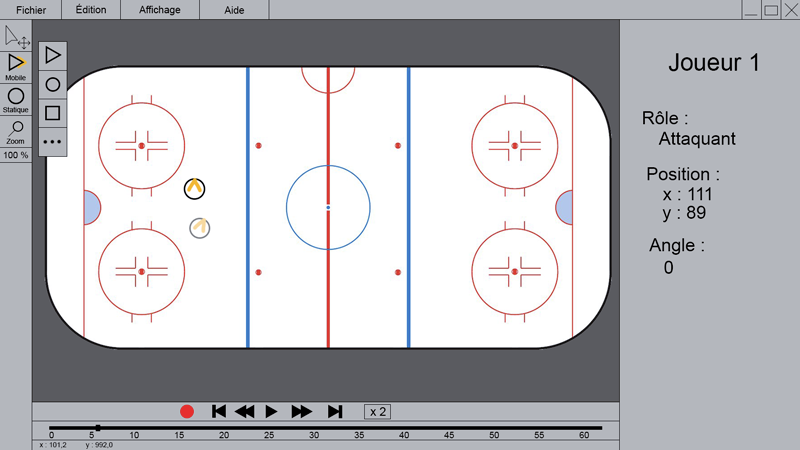
\includegraphics[width=\textwidth]{mockup/mockup.png}
	\caption{Maquette principale de l'application}
	\label{fig:mock-up}
\end{figure}

\subsection{Section du centre}

Cette section est celle où la scène est affichée. Dans le fond de la scène s'affiche le terrain. C'est dans cette section que les éléments sont placés. En plaçant la souris sur un élément, une icône s'affiche. En appuyant dessus, il est possible de modifier l'angle de l'élément.

\subsection{Section de droite}

Cette section contient les paramètres de l'élément actuellement sélectionné. Le premier champ, où il est écrit «~Joueur 1~», est le nom de l'élément. Le «~Attaquant~» est le rôle du joueur. C'est une liste déroulante dans laquelle les valeurs sont celles entrées dans les paramètres du sport. La position en x et en y de l'élément est modifiable via des champs numériques. L'angle est aussi modifiable en utilisant une glissière. Notez qu'il n'y a pas de rôle pour les éléments statiques et les balles, mais que leurs attributs sont tout de même modifiable dans cette interface.

\subsection{Section du bas}

Cette section permet de gérer la visualisation de la stratégie. Le cercle rouge permet de démarrer l'enregistrement de la stratégie. Les autres boutons sont les boutons traditionnels lors du visionnement de vidéo. Le \textit{x2} est dans un champ numérique. En changeant sa valeur, on modifie la vitesse de défilement lors d'avance rapide et de recul. Notez que le «~x~» est seulement présent pour l'affichage. Lorsque l'on édite le champ, il n'est pas présent.

En dessous se trouve une ligne du temps. Le rectangle noir, le curseur, indique quelle image est affichée dans la scène. En le modifiant, l'image affichée dans la scène change. On peut voir juste en dessous la position en x et en y de la souris.

\subsection{Section de gauche}

Cette section contient les boutons permettant d'ajouter des éléments à la scène. C'est la barre d'outils. Le premier à partir du haut est celui utilisé pour déplacer les éléments. Le second sert à créer les éléments mobiles. Le troisième sert à créer les éléments statiques. En maintenant un clic sur le second et le troisième bouton, des icônes apparaissent à droite. Ils permettent de modifier l'élément qui sera ajouté à la scène grâce aux outils d'ajout d'éléments. Le quatrième bouton sert à zoomer sur la scène. Juste en dessous se trouve un champ numérique, permettant de modifier le zoom. La molette de la souris permet aussi de réaliser cette tâche.

\subsection{Menu}

Le menu se retrouve en haut complètement. À l'intérieur de ces menus, on retrouve les commandes pour charger et sauvegarder la stratégie, les commandes qui permettent d'annuler ou de rétablir la dernière action ainsi que différentes options d'affichage. C'est à partir de ce menu que l'on peut charger l'éditeur de sport. La grande majorité de ces commandes ont des raccourcis claviers afin de permettre leur utilisation rapide.

\section{Fenêtre de configuration de sport}

\begin{figure}[H]
	\centering
	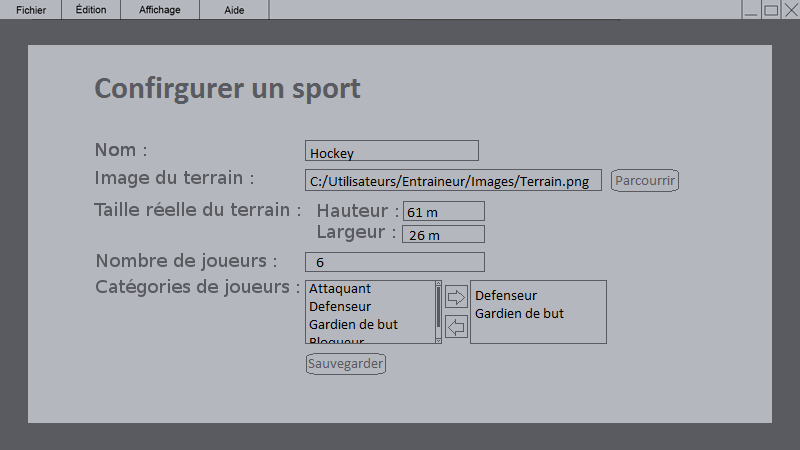
\includegraphics[width=\textwidth]{mockup/mockupSport.png}
	\caption{Maquette de l'écran dde configuration de sport}
	\label{fig:mock-up-sport}
\end{figure}

\subsection{Description}

La figure \ref{fig:mock-up-sport} présente la fenêtre d'édition du sport. Cette fenêtre est accessible via les menus de la fenêtre principale.

Elle est constituée d'un formulaire qui permet d'entrer le nom du sport, de spécifier l'image utilisée comme arrière-plan et les dimensions du terrain. Il permet aussi de modifier le nombre de joueurs et de choisir les rôles des joueurs pouvant faire partie du sport.
\chapter{Échéancier}
\label{s:echeancier}

La figure \ref{fig:gantt} présente l'échéancier actuel du projet sous la forme d'un diagramme de Gantt. Les principales activités ainsi que les livrables y sont identifiées.

\begin{figure}[p]
	\centering
	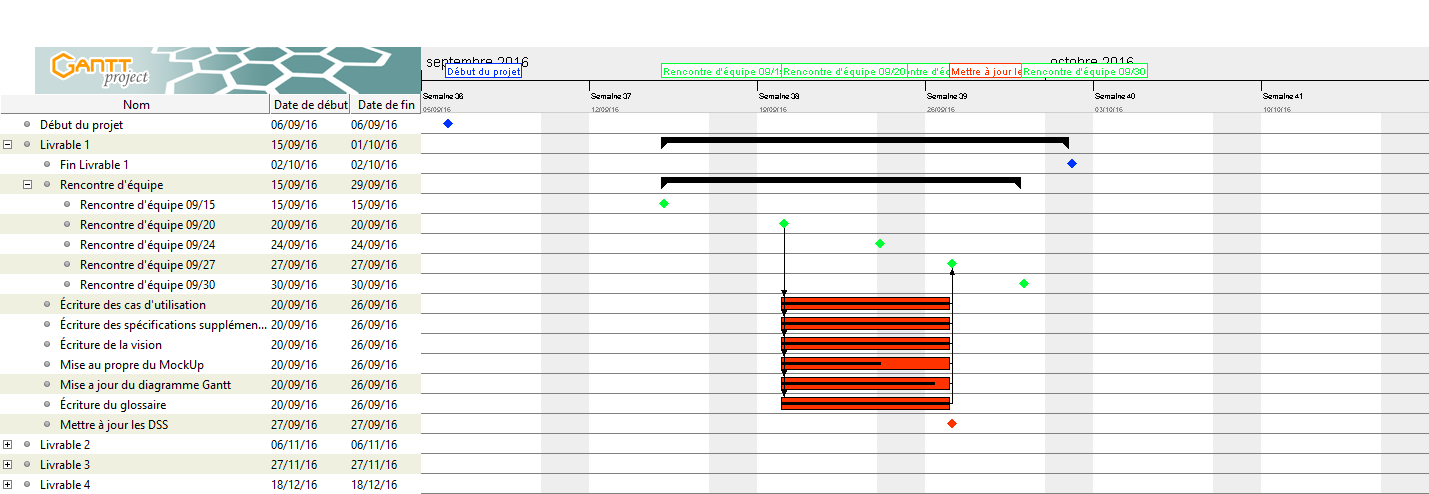
\includegraphics[width=\textwidth, angle=90]{fig/gantt.png}
	\caption{Échéancier du projet}
	\label{fig:gantt}
\end{figure}

% Appendices
\appendix
\chapter{Glossaire}
\label{s:glossaire}

\begin{tabular}{|l|p{12cm}|}
	\hline
	Nom & Définition \\
	\hline
	Scène 				& Section principale de l'écran. C'est dans cette section que l'aire de jeu et les éléments sont affichés. \\
	Stratégie  			& Ensemble des joueurs et de leurs déplacements dans la scène. \\
	Élément 			& Objet qui peut être placé dans la scène. \\
	Élément statique 	& Élément qui ne se déplace jamais dans la scène. \\
	Élément mobile 		& Élément qui peut se déplacer dans la scène (ex~: un joueur ou une rondelle). \\
	Joueur				& Élément mobile représentant un membre d'une équipe sportive. \\
	Type de sport		& Ensemble de propriétés définissant un sport telles que les dimensions du terrain ou le nombre de joueurs. \\
	Curseur 			& Élément visuel se déplaçant horizontalement sur la ligne du temps indiquant l'image actuellement affichée sur la scène. \\
	Ligne du temps 		& Section de l'écran où l'on retrouve une représentation visuelle de la progression temporelle de la stratégie. \\
	Image				& Rendu de la scène à un moment donné dans le temps. \\
	Barre d'outils 		& Section de l'écran où sont situés les boutons permettant de placer ou déplacer les éléments. \\
	\hline
\end{tabular}


\end{document}
